\documentclass{report}

% Language setting
% Replace `english' with e.g. `spanish' to change the document language
\usepackage[english]{babel}

% Set page size and margins
% Replace `letterpaper' with `a4paper' for UK/EU standard size
\usepackage[letterpaper,top=2cm,bottom=2cm,left=3cm,right=3cm,marginparwidth=1.75cm]{geometry}

% Useful packages
\usepackage{amsmath}
\usepackage{graphicx}
\usepackage{float}
\usepackage{subcaption}
\usepackage{chronology}
\usepackage[colorlinks=true, allcolors=blue]{hyperref}

\newtheorem{definition}{Definition}[section]

\title{Protein Data Bank and File Formats}
\author{Vinay Kakkar}

\begin{document}
\maketitle

\tableofcontents

\begin{abstract}


\end{abstract}

\renewcommand\thesection{\arabic{section}}

\section{Protein Data Bank}

The Protein Data Bank was established at Brookhaven National Laboratories ~\cite{bernstein_protein_1977} in 1971 as an archive for biological macromolecular crystal structures~\cite{berman_protein_2000}.

\begin{definition}[Macromolecular]
    Macromolecular is any very large molecule, usually with a diameter ranging from about 100 to 10,000 angstroms
\end{definition}

It is a information source for data retreved from with atomic structures, crystallography and three-dimensional structures of biomolecules, including nucleic acids and proteins~\cite{behzadi_worldwide_2021}. 

At the time this was the first open-access digital dataresource in biology which started with just seven protein structures~\cite{burley_rcsb_2022}.

Various groups such as the Protein Data Bank in Europe, Protein Data Bank Japan help manage the Protein Data Bank archive. Current wwPDB members also include the ElectronMicroscopy Data Bank and the Biological Magnetic Resonance Bank~\cite{burley_rcsb_2022}.

Protein Data Bank China has recently joined the wwPDB as an Associate Member with its role as wwPDBdesignated PDB Archive Keeper. Where they are responsible for weekly updates of the archive and safeguarding both digital information and a physical archive of correspondence~\cite{burley1_rcsb_2022}.

The management of PDB must comply with FAIR (the acronym depicts: Findable, Accessible, Interoperable, Reusable) and FACT~\cite{van_der_aalst_responsible_2017} guiding principles for scientific data~\cite{wilkinson_fair_2016}~\cite{westbrook_impact_2020}.

\begin{table}[h!]
    \begin{center}
    \label{tab:FAIR}
        \begin{tabular}{c|p{0.65\linewidth}}
        The FAIR Guiding Principles\\
        \hline
        \\
        To be Findable: & F1. (meta)data are assigned a globally unique and persistent identifier\\
        & F2. data are described with rich metadata (defined by R1 below)\\ & F3. metadata clearly and explicitly include the identifier of the data it describes\\ & F4. (meta)data are registered or indexed in a searchable resource\\
        \\
        \hline
        \\
        To be Accessible: & A1. (meta)data are retrievable by their identifier using a standardized communications protoco\\
        & A1.1 the protocol is open, free, and universally implementable\\ & A1.2 the protocol allows for an authentication and authorization procedure, where necessary\\ & A2. metadata are accessible, even when the data are no longer available
        \\
        \hline
        \\
        To be Interoperable: & I1. (meta)data use a formal, accessible, shared, and broadly applicable language for knowledge representation.\\
        & I2. (meta)data use vocabularies that follow FAIR principles\\ & I3. (meta)data include qualified references to other (meta)data\\
        \\
        \hline
        \\
        To be Reusable: & R1. meta(data) are richly described with a plurality of accurate and relevant attributes\\
        & R1.1. (meta)data are released with a clear and accessible data usage license\\ & R1.2. (meta)data are associated with detailed provenance\\ &
        R1.3. (meta)data meet domain-relevant community standards\\
        \end{tabular}
        \caption{\label{Fair}The guidlines to what builds up the FAIR principles~\cite{wilkinson_fair_2016}}
    \end{center}
\end{table}

\subsection{Aims and Objectives of PDB}

Enzymology, electron microscopy, computational chemistry small molecule crystallography, biochemistry, biophysics, macromolecular crystallography and nuclear magnetic resonance spectrometry all help the aims and goals of the PDB archive.

supports the structural biology as the front line aim and goal of the PDB archive [19]~\cite{behzadi_worldwide_2021}

\begin{definition}[Enzymology]
    Enzymology is the branch of biochemistry aiming to understand how enzymes work
\end{definition}

\begin{definition}[Electron Microscopy]
    Electron microscopy is a technique for obtaining high resolution images of biological and non-biological specimens.
\end{definition}

PDB's provides open access to nearly 200 000 archived, validated and biocurated experimentaly determined three-dimensional structures of biological macromolecules.3D structures archived in the PDB have enabled important scientific breakthroughs by basic and applied researchers~\cite{burley_impact_2021}. Open access to PDB data without restrictions on usage has also aided structural bioinformatics to areas such as computational biology.

\subsection{Timeline of PDB}

I have provided a timeline representing the milesstones achived within the protein data bank. Where PDB marked its 52st anniversary of continuous operations.

\begin{chronology}{1971}{1981}{90ex}
    \event{1971}{PDB established}
    \event{1973}{Early structures include}
    \event{1974}{First tRNA structures}
    \event{1979}{First Z-DNA published}
    \event{1981}{First B-DNA in the PDB}
\end{chronology}

\begin{chronology}{1989}{2001}{90ex}
    \event{1989}{IUCr policy and First NMR structure}
    \event{1991}{First 3DEM structure}
    \event{\decimaldate{1}{11}{1994}}{First PDB Web Browser}
    \event{\decimaldate{1}{5}{1996}}{25th Anniversary and Release of AutoDep}
    \event{\decimaldate{1}{10}{1998}}{10,000th structure is released}
    \event{2000}{Osaka center and First ribosome structures}
    \event{\decimaldate{1}{7}{2001}}{EMDB established at MSD-EBI}
\end{chronology}

\begin{chronology}{2003}{2011}{90ex}
    \event{2003}{wwPDB established by RCSB, PDBe, PDBj}
    \event{\decimaldate{1}{10}{2004}}{Last postal PDB archive}
    \event{2006}{BMRB joins wwPDB}
    \event{\decimaldate{1}{11}{2006}}{First release of remediated data}
    \event{\decimaldate{1}{7}{2008}}{50,000th structure and Deposition of (X-ray, NMR)}
    \event{\decimaldate{1}{10}{2009}}{Deposition chemical shift and Worldwide PDB Foundation established}
    \event{2011}{PDB40 Symposium and First structure X-ray Free Electron Laser}
\end{chronology}

\begin{chronology}{2012}{2021}{90ex}
    \event{\decimaldate{1}{5}{2012}}{Validation Reports}
    \event{\decimaldate{1}{4}{2013}}{Large structures PDBx/mmCIF}
    \event{2014}{OneDep and 100,000+ structures}
    \event{\decimaldate{1}{3}{2015}}{Reports NMR, 3DEM and Deposition of EM maps}
    \event{\decimaldate{1}{4}{2016}}{PDB-Dev and PDB Entry Versioning}
    \event{\decimaldate{1}{2}{2017}}{ligand validation and 150,000+ structures}
    \event{\decimaldate{1}{11}{2018}}{First SARS-CoV-2 structure }
    \event{\decimaldate{1}{6}{2019}}{Reports for 3DEM coord, maps}
    \event{\decimaldate{1}{12}{2019}}{Alphafold2 and carbohydrate data}
    \event{2021}{PDB50 and EMDB partner in wwPDB}
\end{chronology}

\subsection{Recent Project}

A project was undertaken to change the information management services for RCSB.org. The idea is was to have developed a primary place for studying 3D biostructures by extending RCSB.org web portal functionality to support parallel delivery of more than one million CSMs publiclyavailable from AlphaFold DB and ModelArchive together~\cite{burley1_rcsb_2022}.

\subsection{Covid}

During COVID-19 pandemic more than 2000 structures associated with the agent of the coronavirus disease were released and have become accessible for global users for free. The properties of these structures give us this opportunity to find out the ligand binding sites, spatial conformation of ligands, protein to protein interactions and amino acid substitutions regarding different viral proteins. Moreover, hemical, functional and energetic characteristics can also be gained from to describe the potential capabilities for each individual molecule. These properties might aid us to determine the potential drug targets for drug design and vaccine preparation~\cite{lubin_evolution_2020}.

\subsubsection{Example case on why PDB is important}

210 new molecular entities were discovered and developed during a period of 2010 to 2016 which were approved by the US Food and Drug Administration. The primary 3D structural data and information of these NMEs compartments, were first produced and released into the PDB archive. The representation of the related structures encouraged pharma companies to finance in drug discovery and development~\cite{westbrook_impact_2020}~\cite{westbrook_how_2019}~\cite{behzadi_worldwide_2021}

\section{PDB Currently}

As of 2022, the PDB has a vast number of 3D biostructures, eukaryotic protein structures exceeded 105 000. Bacterial protein structures were also numerous, totaling nearly 66 000. Archaeal protein structures were the least numerous totaling 5500. However the PDB coverage is decidedly limited, with mouse protein structures being most numerous at 8000 structures~\cite{burley_open-access_2021}. 

We have powerful tools developed by RCSB PDB for searching and analysis which include structure, sequence, sequence motif, structure motif, and visualization~\cite{burley1_rcsb_2022}.

Upon reaching the RCSB.org home page, users can query, organize, visualize, analyse, compare, and explore PDB structures and CSMs side-by-side. Searching 3D structure information can encompass PDB structures and CSMs or be limited to PDB structures only. Either PDB structures or CSMs can be excluded from the search results. The two types of structure information accessible via RCSB.org are clearly distinguished from each other. Top bar searching and data delivery for PDB structures and CSMs~\cite{burley1_rcsb_2022}.

\subsubsection{The PDB Site currently}

\begin{figure}[H]
    \centering
    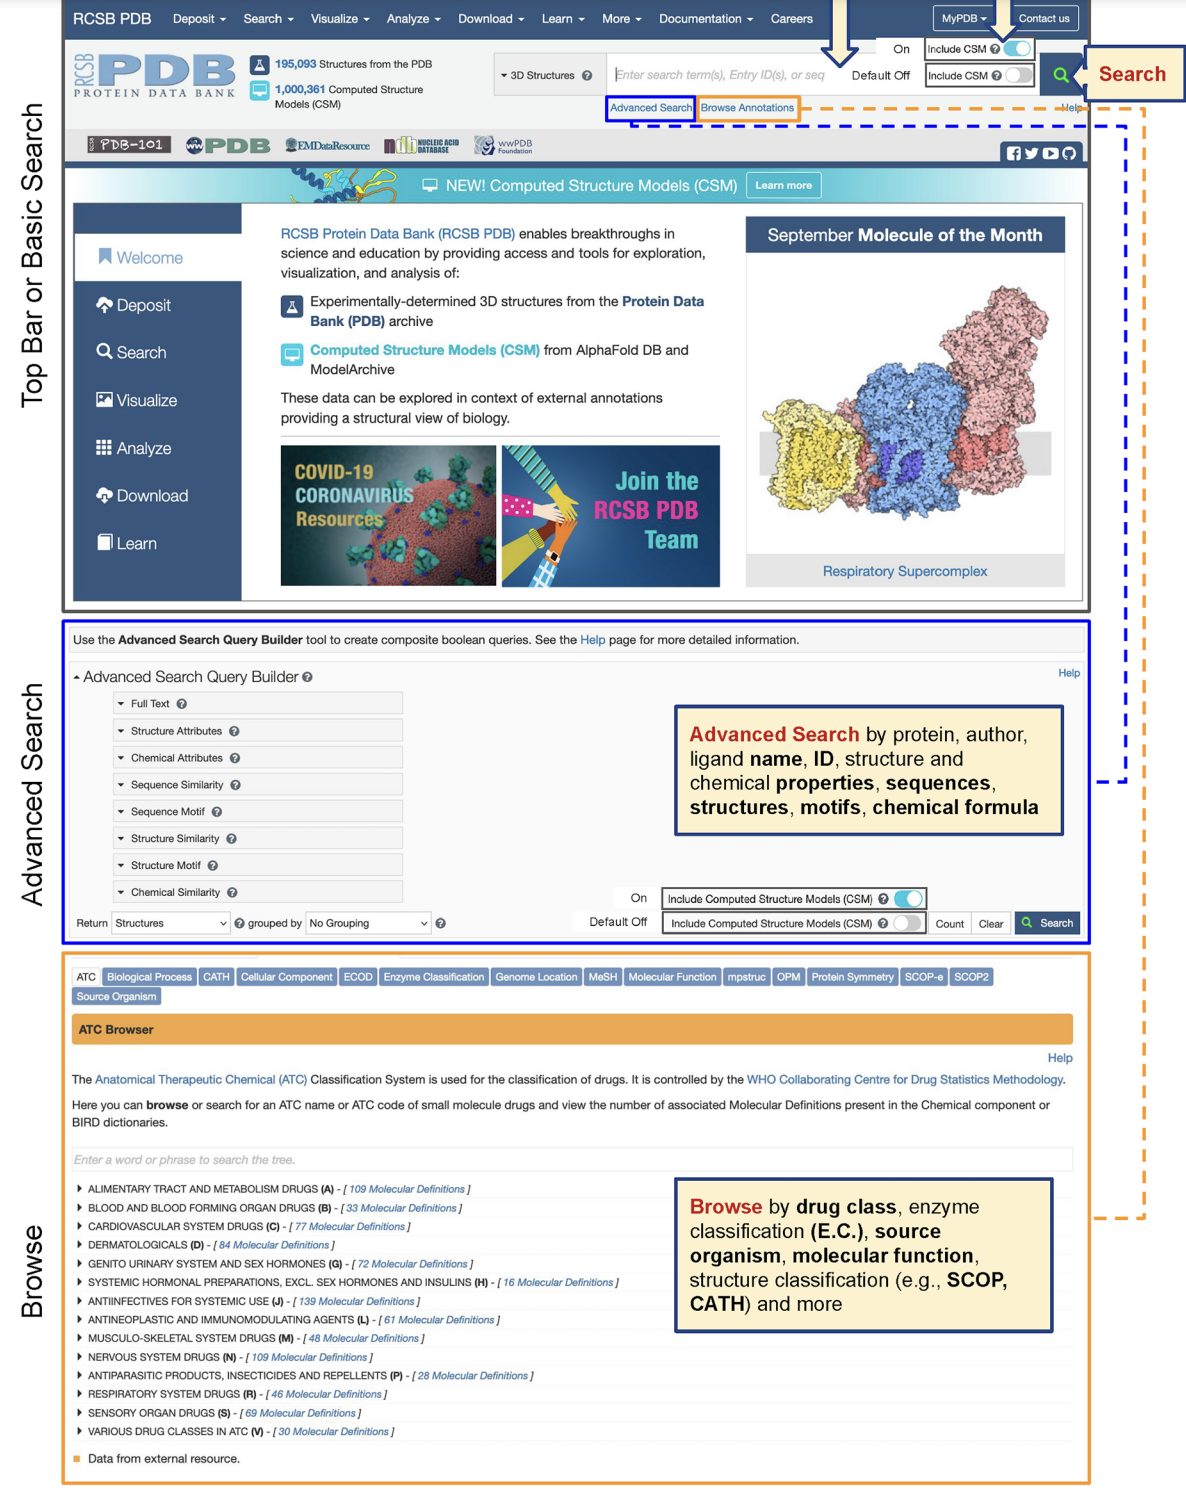
\includegraphics[width=0.5\textwidth]{PDB Site.png}
    \caption{\label{fig:PDB}Search options at RCSB.org include Top Bar or Basic Search; Advanced Search; and Browse Annotations~\cite{burley1_rcsb_2022}.}
\end{figure}

\begin{figure}[!h]
    \centering
    \begin{subfigure}[t]{.45\textwidth}
        \centering
        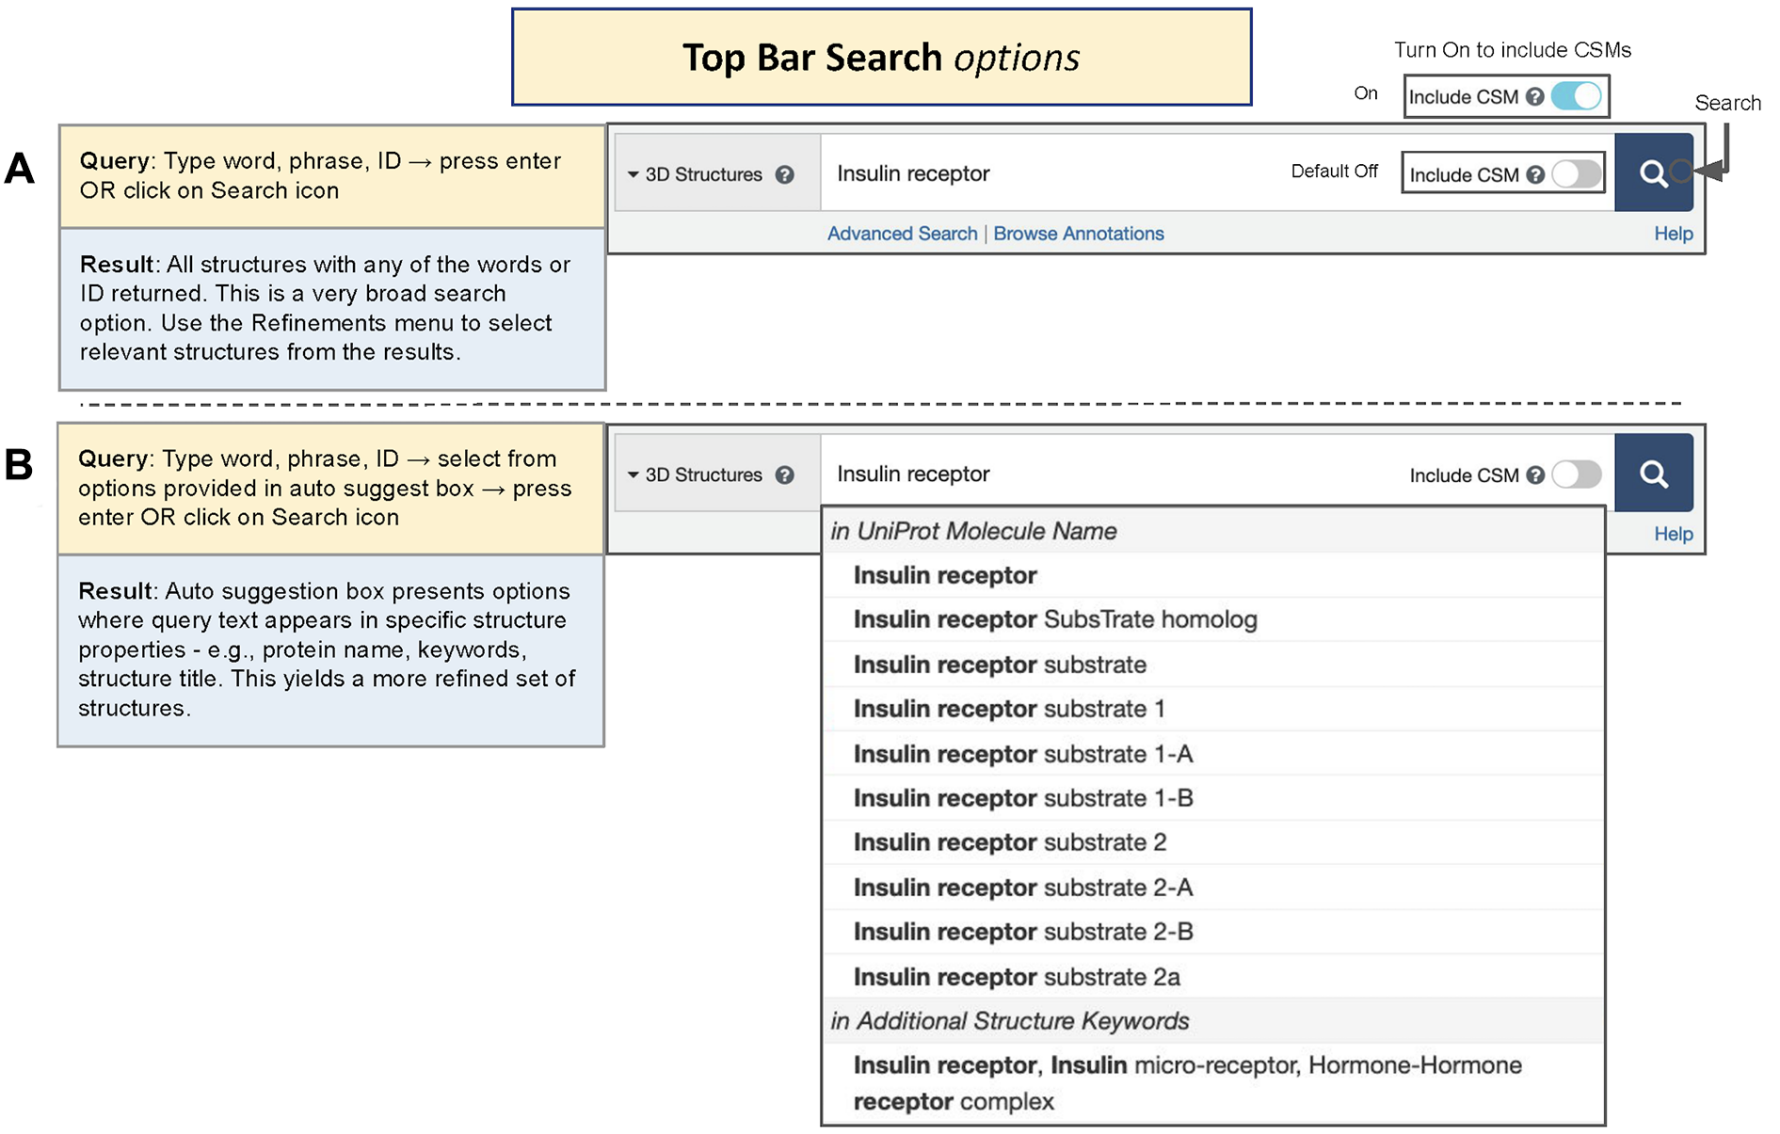
\includegraphics[width=0.9\textwidth]{Top Bar Search A.png}
        \caption{}
        \label{fig:Top1} 
    \end{subfigure}
    \begin{subfigure}[t]{.45\textwidth}
       \centering
       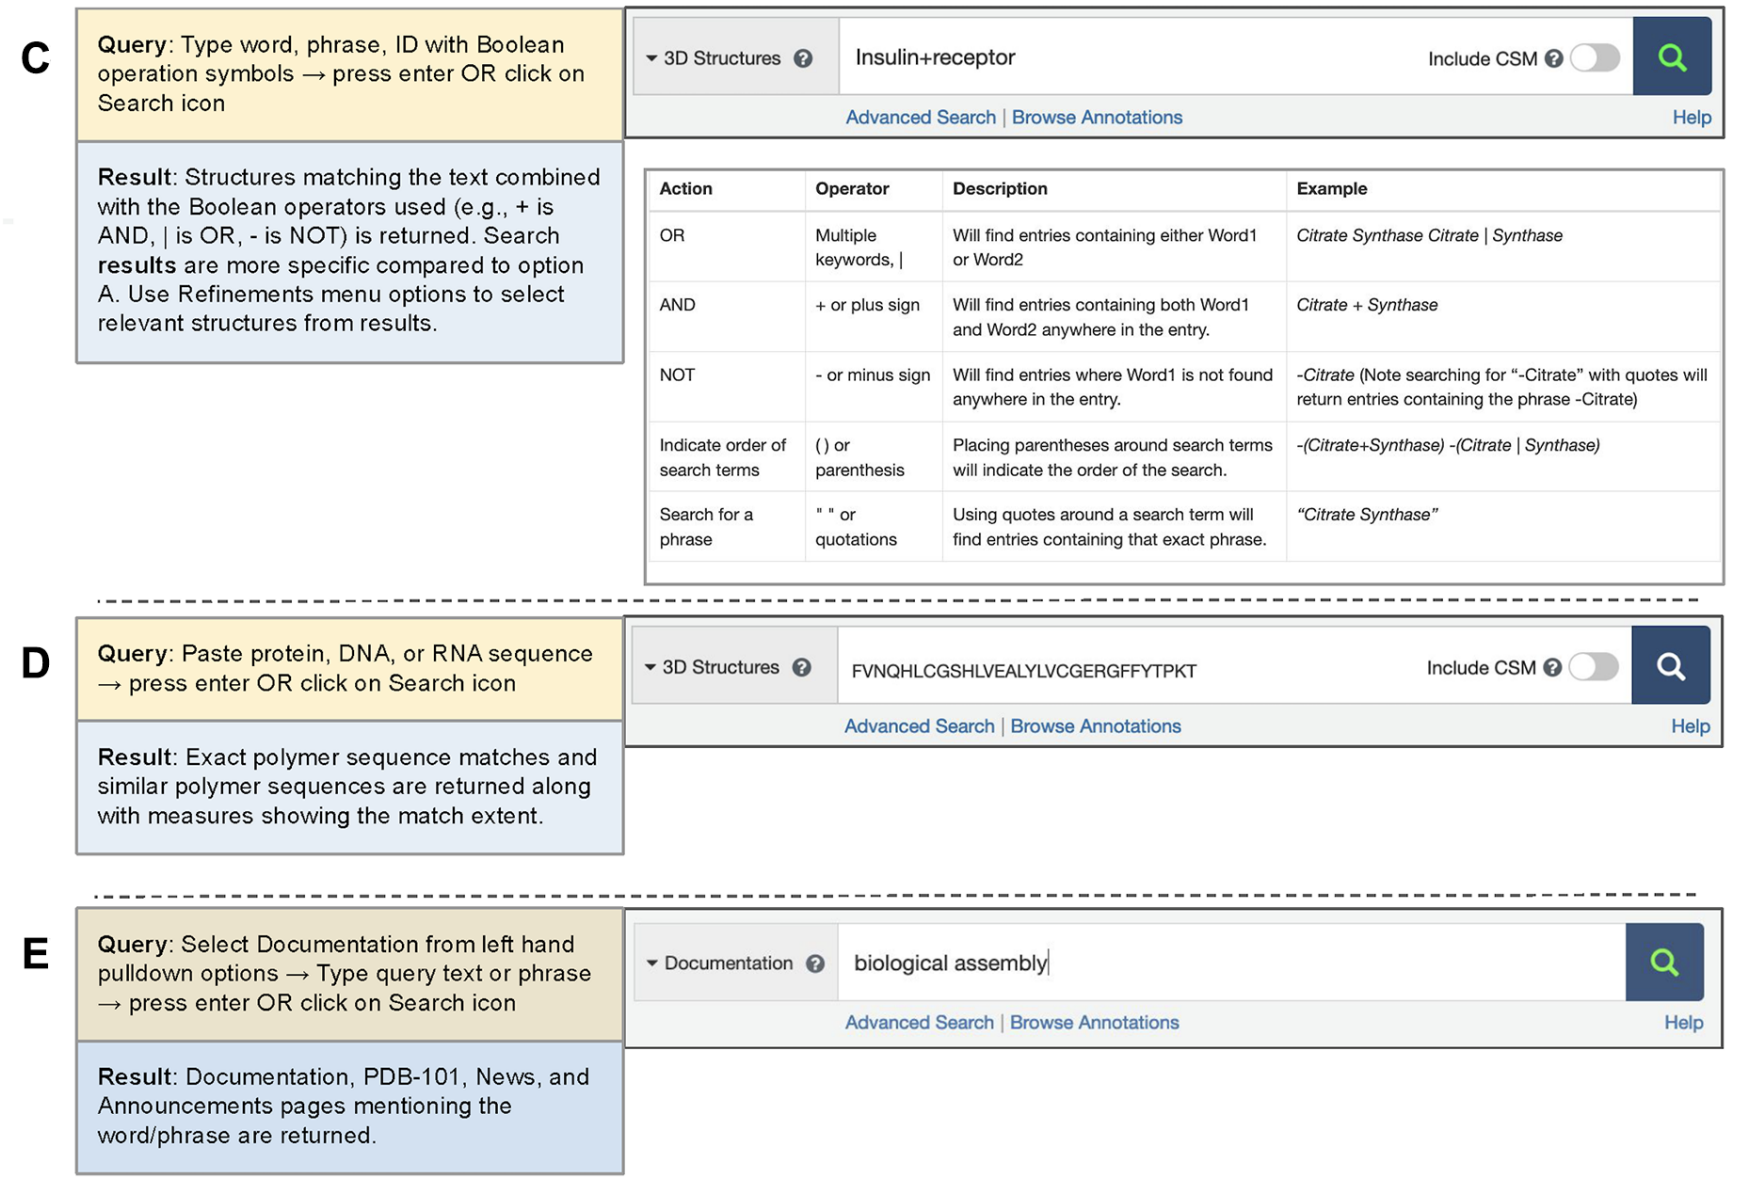
\includegraphics[width=0.9\textwidth]{Top Bar Search B.png}
       \caption{}
       \label{fig:Top2}
    \end{subfigure}
    \caption{\emph{Top Bar or Basic Search options available from every RCSB.org web page. Examples of searching for 3D structures using (A) simple text string insulin receptor; (B) drop down autosuggestions based on the text string insulin receptor; (C) Boolean operators to combine insulin + receptor (+ = AND); or (D) an amino acid sequence. (E) Searching RCSB.org documentation using a text string biological assembly~\cite{burley1_rcsb_2022}}}
    \label{fig:SAGE}
\end{figure}


The site has some key navigational features that provide users with access to Top Bar Search on the RCSB.org home page, Advanced Search, and Browse Annotations. The default option searches PDB structure data only. CSMs can be included with the toggle switch. Entering a keyword (e.g., molecule name, database entry ID (PDB, UniProt, AlphaFold DB, ModelArchive), author name (PDB structures only)) will launch autosuggestions organized by data category. Sequence searches can be run by entering single-letter code sequences for protein, DNA or RNA polymers and executing the query. Top Bar Search can also be used to search documentation and news announcements available on both RCSB.org and the RCSB PDB outreach by changing the search type from 3D Structures to Documentation on the left of the search box~\cite{burley1_rcsb_2022}.

\section{Recent Improvements}

\subsection*{Recent RCSB PDB data architecture improvements}

In 2020, RCSB PDB had a upgrade of its delivery architecture~\cite{rose_rcsb_2021}at RCSB.org~\cite{powerful_rcsb_2021}. The legacy monolithic data delivery application  was changed into a distributed deployment of individual microservices, each with a single responsibility. Data access services provide both Representational State Transfer and GraphQL API access to a data warehouse hosted in a MongoDB  documentoriented database. Originaly, advanced Search QueryBuilder functionality encompassed text, PDB data attributes, 3D structure, sequence, biopolymer sequence motif, and chemical similarity. Every search function is implemented as an independent service. A separate search service is responsible for launching each search function, combining and delivering their integrated results to public programmatic search APIs. When each service has a single responsibility, we have a greater flexibility in scaling the deployment of services in response to changes in user load and significant reductions in the time required to develop, test, and deploy new features. The Sequence Motif search function has been extended with a new 3D Structure Motifsearch capability~\cite{bittrich_real-time_2020}. 

Chemical Search function now has the ability to perform exhaustive substructure searching across the small molecules represented in the PDB archive, managed by the search Aggregator service and available through our public search APIs. To monitor the new service architecture, there is a system for processing service logs and indexing the time of request all whilst respecting PDB data consumer privacy. These statistics can be used to aid in monitoring the health of RCSB PDB production services~\cite{burley_rcsb_2022}.

\subsection*{Recent advances in RCSB PDB data integration}

RCSB PDB integrates the content of each expertly biocurated Entry with information from more than 50 external data resources. 

Intergrated external data needs to follow a data schema that defines the organization of the RCSB PDB data warehouse. Finally it is  available to RCSB PDB front end services, public data access APIs, and our text search indexing service~\cite{burley_rcsb_2022}.

\begin{table}[h!]
    \begin{center}
    \label{tab:External Data}
        \begin{tabular}{c|p{0.58\linewidth}}
        External Resources\\
        \hline
        \\
        AlphaFold DB & Computed Structure Models by AlphaFold2
        \\
        \hline
        \\
        ATC & 	Anatomical Therapeutic Chemical (ATC) Classification System from World Health Organization
        \\
        \hline
        \\
        Binding MOAD & Binding affinities
        \\
        \hline
        \\
        Binding DB & Binding affinities
        \\
        \hline
        \\
        BMRB & BMRB-to-PDB mappings
        \\
        \hline
        \\
        Cambridge structural Database & Crystallographic small molecule data from the Cambridge Crystallographic Data Centre
        \\
        \hline
        \\
        CATH & 	Protein structure classification- Class, Architecture, Topology/fold, and Homologous superfamily    
        \\
        \hline
        \\
        ChEMBL & Manually curated database of bioactive molecules with drug-like properties
        \\
        \hline
        \\
        CSD & Cambridge Structural Database: Validated and curated small-molecule organic and metal-organic crystal structures from the Cambridge Crystallographic Data Centre
        \\
        \hline
        \\
        DrugBank & Drug and drug target data
        \\
        \hline
        \\
        ECOD & Evolutionary Classification of Protein Domains
        \\
        \hline
        \\
        EMDB & 3DEM density maps and associated metadata
        \\
        \hline
        \\
        ExplorEnz & IUBMB Enzyme nomenclature and classification
        \\
        \hline
        \\
        Gencode & Human and Mouse Gene annotations
        \end{tabular}
        \caption{\label{External Data}Some of the External Resources Integrated Into RCSB PDB}
    \end{center}
\end{table}



\subsection*{Recent PDBx/mmCIF data standard improvements}

The PDBx/mmCIF data standard is maintained by the wwPDB organization in collaboration with wwPDBPDBx/mmCIF Working Group domain experts recruited from the scientific community. The PDBx/mmCIF web resource supports browse and search access to standard terminology. The Working Group includes developers for many of the widely used structure determination software systems, who ensure that data produced by these programs comply with the PDBx/mmCIF data standard, generating complete and correct data files for PDB deposition. The wwPDB and the Working Group collaborate on developing terminologies for new and rapidly evolving methodologies such as Free Electron Laser, 3DEM, Serial Crystallography, and X-ray, whilst improving representations for existing data content. Most recently, the Working Group has focused on modernizing content descriptions for processed X-ray diffraction data, including extensions describing anisotropic diffraction limits, unmerged reflection data, and new quality metrics of anomalous diffraction data. Deposition and delivery improve our ability to assess experimental data quality, and every PDB data consumer's ability to Find and Reuse relevant PDB Entries~\cite{burley_rcsb_2022}.

\subsection*{Mol* molecular graphics visualization}

PDB data provides 3D shapes and interactions of biological macromolecules where we ultimatly would like to understand the biological function. 

Mol* was deployed in 2020~\cite{sehnal_mol_2021} and set as the default RCSB.org molecular graphics tool for visualizing. This software system was developed as a community project, co-led by RCSB PDB and the Protein Data Bank in Europe. 

Mol* graphics tool is used for interrogating 3D macromolecular structure data from the PDB or computed structure models. It works entirely within the PDB site. Mol* also supports integration of information from other bioinformatics resources. These insights can help develop new hypotheses for research and facilitate analysis. Overall it allows to easily visualize entire polypeptide or nucleic acid chains, whole biological Assemblies, or specific atoms or groups of atoms ina particular biological macromolecule it can also display molecular surfaces, and noncovalent interactions with bound ligands, ions, drugs, and inhibitors~\cite{burley_rcsb_2022}.

\section{Summary}
\subsection{Future and struggles of PDB}
\subsubsection{Future}
As the PDB archive has started its 52nd year, it gives open acess to analyses of strucutres and much more to: basic and applied researchers, educators, and students spanning fundamental biology, biomedicine, bioenergy, bioengineering and biotechnology, with key points that help many communities that use this ficlity. Firstly It delivers Data In and Data Out services efficiently to a user base that is now numbering many millions worldwide. Secondly it has wwPDB partners that process, validate, and biocurate the growing number of increasingly complex PDB depositions received. Manages and safeguards the growing PDB archive in its role as wwPDB designated Archive Keeper. Thirdly it enables searching, visualization, exploration and analysis of experimentally-determined PDB structures integrated with more than one million CSMs through its web portal. Lastly it supports user training, education, and outreach through PDB101.RCSB.org.~\cite{burley1_rcsb_2022}.

\subsubsection{Struggles}
Even after all the advancments PDB has gone through there are still additional challenges lying ahead which include:

\begin{itemize}
    \item Rapid growth in public-domain CSMs of individual polypeptide chains, already numbering >200 million at the time of writing.
    \item Anticipated advances in AI/ML-based prediction of structures of multi-protein complexes.
    \item Continued development of biomolecular structure determination methods using X-ray Free Electron Lasers, revealing the microscopic details of chemical reactions in real time.
    \item Growth in the number and complexity of atomic-level cryoelectrontomography structures of macromolecular machines.
    \item Integration of PDB structures and CSMs with complementary information coming from correlative light microscopy and related imaging methods across length scales ranging from atoms to small molecules to individual biomolecules to macromolecular assemblies to organelles to cells and ultimately tissues
    \item Merging of the PDB-Dev prototype archiving system for integrative methods structures with the PDB archive
    \item Federating other biodata resources, such as the SmallAngle Scattering Database and the Proteomics Identification Database, with the PDB, EMDB and BMRB core archives jointly managed by the wwPDB partnership
\end{itemize}
~\cite{burley1_rcsb_2022}.

\section{File Formats}

The PDB archive holds a few different types of file types which hold data such as atomic coordinates and other information describing proteins and other biological macromolecules. Depending on what the data is created from it can fall into a different category.

\subsection{PDB Data}

The main information in the PDB archive is coordinate files for biological molecules. These files list the atoms in each protein, and their 3D coordinates.

These files are available in several formats:

\begin{itemize}
    \item PDB
    \item mmCIF
    \item XML
\end{itemize}

The header section of text summarizes the protein, citation information, and the details of the structure solution, which is then followed by the sequence and a long list of the atoms and their coordinates. It also contains the experimental observations used to deterimne atomic coordinates~\cite{noauthor_pdb101_nodate}.

\subsubsection{.pdb Files}

The PB format consists of a collection of fixed format records that describe the atomic coordinates, chemical and biochemical features, experimental details of the structure determination. and some structural features such as secondary structure assignments. hydrogen bonding, and biological assemblies and active sites~\cite{westbrook_pdb_2003}.

Each item of data in the PDB format is assigned to a range of character positions in one of many PDB record types (HEADER. SOURCE. REMARK, etc.). The ATOM records encode the atomic coordinate data. ATOM records are among the more than 45 named data records in the PDB format. These named has records have suit column-formatting rules~\cite{westbrook_pdb_2003}.

In addressing changes in experimental methodology, the PDB format has been extended with new REMARK records. For example, the organization and information content of REMARK 3 that encodes refinement information has been modified and extended for each new refinement program and program version Although extending REMARK records in this way captures information in a manner that is easy for a human to read, the diversity of organization of this data makes it very difficult to design software that can automatically and reliably extract information from these records Data m these records is also defined only in terms of the program that computed the information~\cite{westbrook_pdb_2003}.

The PB format uses fixed-width fields to represent data, and this restriction places absolute limits on the size of certain items of data. For instance, the maximum number of atom records that can be represented in a single structure model is limited to 99.999 and the field width of the identifier for polymer chains is limited to a single character.Although these restrictions were certainly reasonable when the format was first defined, this is no longer the case. Many large molecular systems, such as the ribosomal subunit structures, cannot be represented in a single PDB entry. These entries must be divided into multiple PB files, seriously complicating their use~\cite{westbrook_pdb_2003}.

\begin{figure}[H]
    \centering
    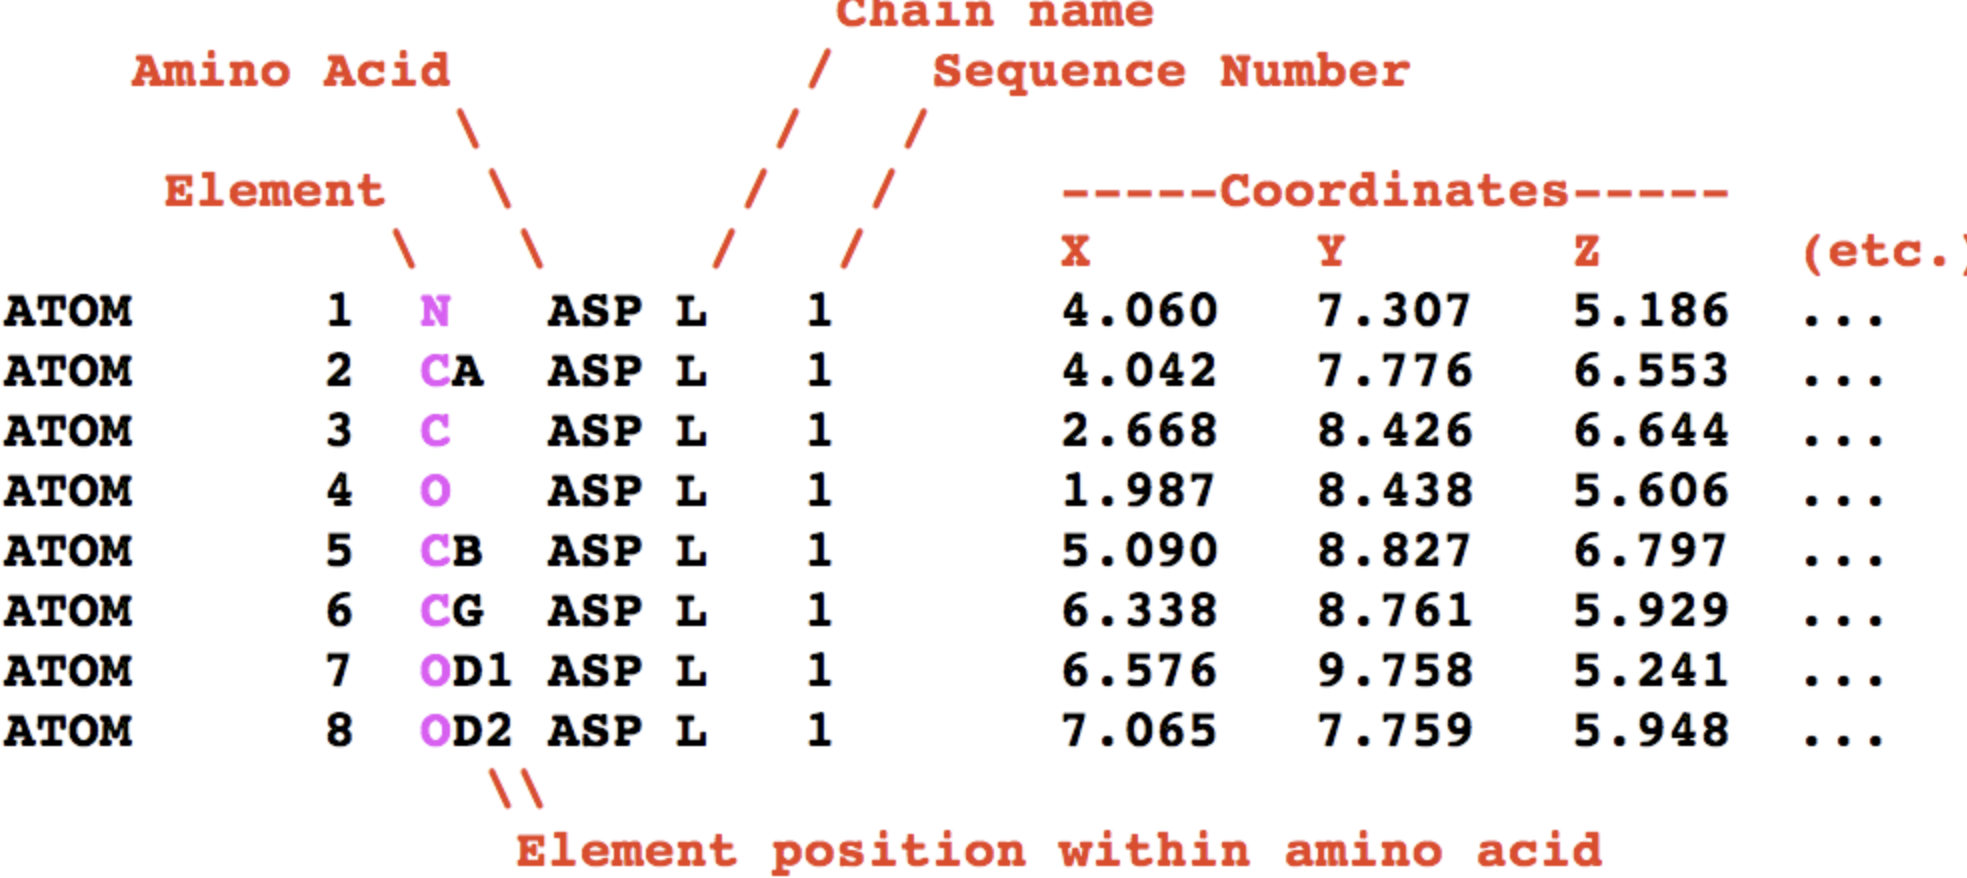
\includegraphics[width=0.5\textwidth]{PDB File.png}
    \caption{\label{fig:PDB file}Showing contents of a PDB file for the Atom values~\cite{adams_announcing_2019}.}
\end{figure}

\subsubsection{.mmCIF Files}
Mmcif is a dictionary based approach to data about crystallographic experiments and results and is the format in which all structures described in articles sent to Act Crystallographic C
are submitted~\cite{westbrook_pdb_2003}.

Implicitly this mandate included the need to describe all the data items included in a PDB entry. Also the need to provide sufficient data names so that the experimental section of a structure paper could be written automatically and to facilitate the development of tools so that computer programs could easily access and validate mmCIF data files~\cite{westbrook_pdb_2003}.

In January 1997, the mmCIF dictionary containing 1700 definitions was completed and submitted to the IUCr committee that oversees dictionary development (COMCIFS) for review and in June 1997. Version 1.0 was released~\cite{westbrook_pdb_2003}.

\subsubsection{.xml}

The representation of PDB data in XML builds from the content of the PDB Exchange dictionary, both for assignment of data item names and for defining data organization. Although presented in very different syntaxes, the PDB Exchange and XML representations use the same logical data organization.

The dictionary data block is mapped to the standard top-level XML schema element, and the data file data block is mapped to a datablock element. The schema and datablock elements provide namespace definitions, linkages to the supporting XML schema definition documents and linkages to the location of the current supporting schema.
Category or table definitions in the Exchange dictionary are
described as XML complexTypes. The category definition and
examples are mapped to XML annotation and documentation elements. The data items within the category are defined as an unordered sequence of XML elements named according to the attribute portion of their dictionary equivalents. The special data items that form the primary key for the category are defined as XML attributes.

\begin{figure}[H]
    \centering
    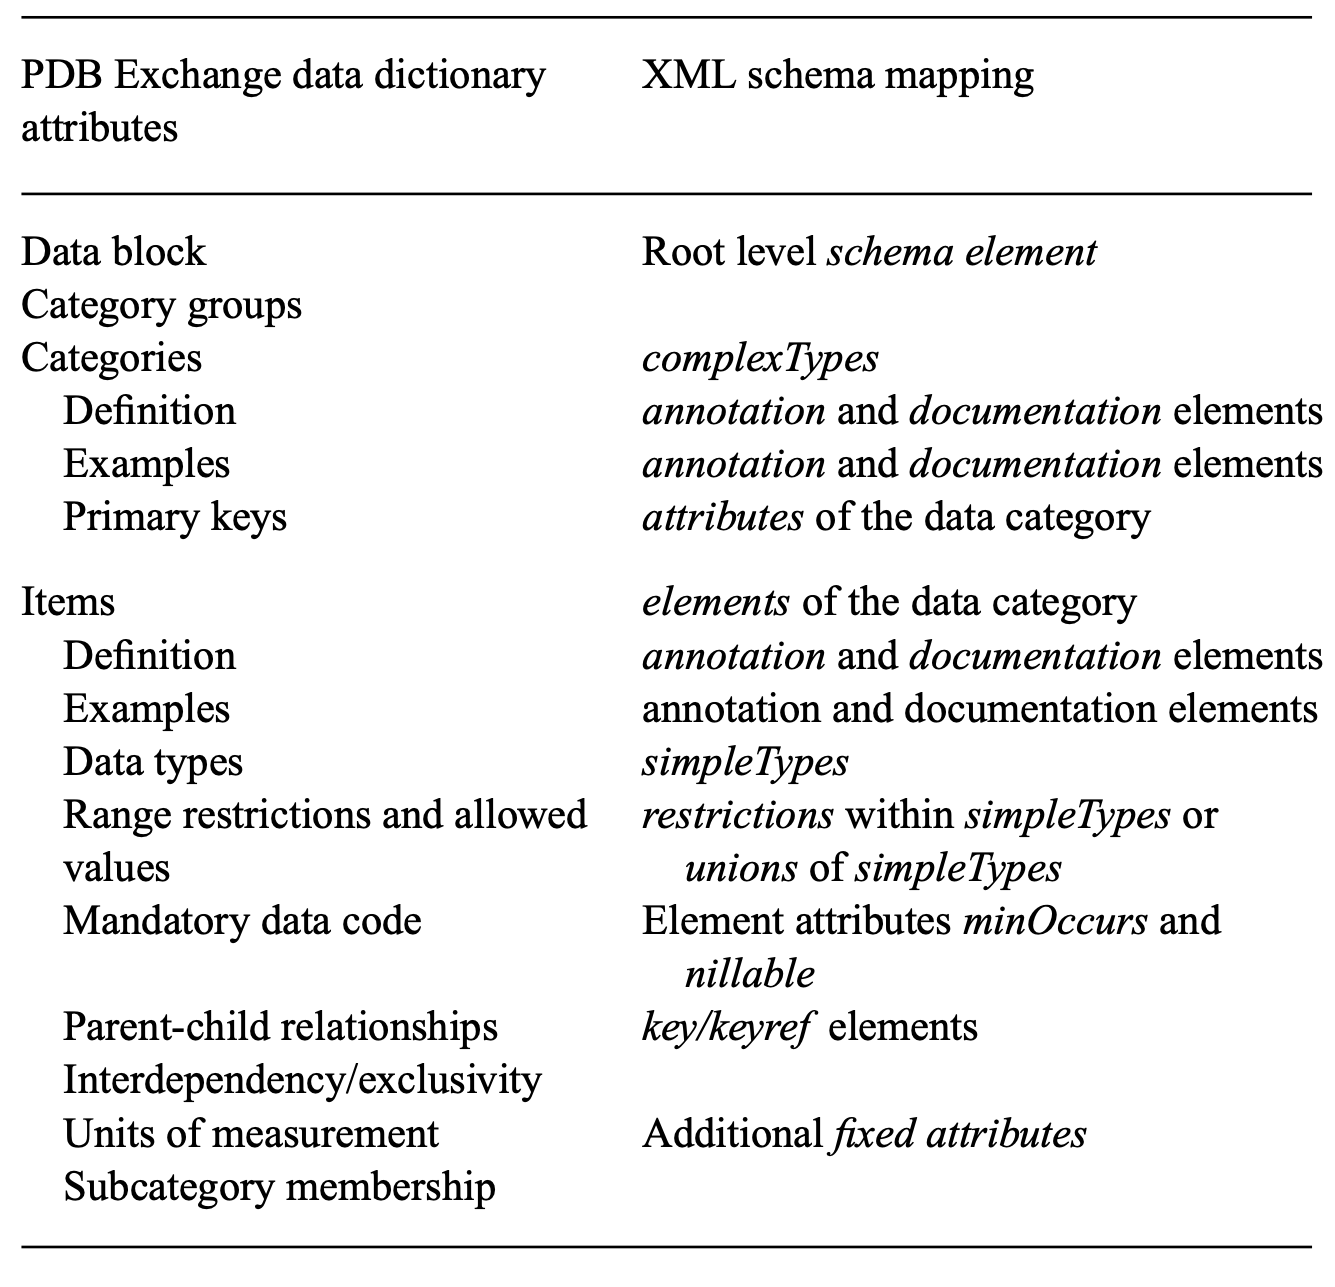
\includegraphics[width=0.5\textwidth]{xml.png}
    \caption{\label{fig:xml}Summary of the correspondences between PDB Exchange data dictionary and XML schema metadata~\cite{westbrook_pdbml_2005}.}
\end{figure}


\subsection{Visualizing Structures}

While you can view PDB files directly using a text editor,
Pdb files can be viewed from text editors but we can also use a browsing or visualization program. RCSB PDB allow you to search and explore the information, including information on experimental methods and the chemistry and biology of the protein. Visualization programs allow to read in the PDB file and, display the protein structure generating custom pictures of it. These programs can contain analysis tools that allow you to measure distances and bond angles, and identify interesting structural features~\cite{noauthor_pdb101_nodate}.

\subsection{Reading Coordinate Files}

Before exploring structures in the PDB archive we need some prior understanding of the coordinate files. For example we can find a diverse mixture of biological molecules, small molecules, ions, and water which can get confusing we can use he names and chain IDs to help sort these out. In structures determined from crystallography, atoms are annotated with temperature factors that describe their vibration and occupancies that show if they are seen in several conformations. NMR structures often include several different models of the molecule~\cite{noauthor_pdb101_nodate}.

\subsection{Potential Challanges}

There are some things to note as you could fall into some challanges when browsing through the PDB archive. Many structures, particular those determined by crystallography, only include information about part of the functional biological assembly. One thing to note is that the PDB can aid with this. Another note is many PDB entries are missing portions of the molecule that were not observed in the experiment. These include structures that include only alpha carbon positions, structures with missing loops, structures of individual domains, or subunits from a larger molecule. In addition, most of the crystallographic structure entries do not have information on hydrogen atoms~\cite{noauthor_pdb101_nodate}.



\bibliographystyle{alpha}
\bibliography{bibliography}


\end{document}